\documentclass[article,oneside]{memoir}

\usepackage{graphicx} % Add graphics capabilities
\usepackage{booktabs} % ``Proper'' table layout
\usepackage{amsmath}  % Better maths support
%\usepackage[colorlinks=false,linkcolor=red]{hyperref} % Hyperlink capabilities
\usepackage{url}

\usepackage{memhfixc} % This package is required to resolve incompatibilities
                      % with the memoir class & the hyperref package
                      
\setlength{\oddsidemargin}{ 20pt}
\setlength{\textwidth}{440pt}
\setlength{\topmargin}{ 0pt}
\setlength{\headheight}{00pt}
\setlength{\headsep}{40pt}
\setlength{\textheight}{620pt}

\title {ENEE631 Assignment 4}
\author{Naotoshi Seo, sonots@umd.edu}
\date{April 18, 2007}


\begin{document}

\maketitle


\chapter{MPEG Video}

\subsubsection{List the parameters you choose for the vector mpg\_option}

\noindent (a) [1 0 0 1 10 2  2 4] achieved PSNR 26.0292 dB $ > $ 26 dB and Bit Rate 1,833,096 bps. 

\noindent (b) [1 0 0 1 10 18 23 28] achieved PSNR 24.0220 dB and Bit Rate 396,936 bps $<$ 400 Kbps

\subsubsection{Give a rule of thumb on how to choose those parameters in step 1}

To increase PSNR (to increase accuracy), decrease quantization scale. 
To increase BIt Rate, reversely, increase quantization scale. Of course, this results in decreasing PSNR. 

We can also change parameters for choice of algorithm to achieve better PSNR or bps, but I did not use them because what I wanted to do here was to make PSNR or bps close to goals gradually. 

\chapter{Motion Estimation and Compensation}

\subsubsection{Draw block diagrams inllustrating the hybrid video encode and decoder based on 
motion compensation and DCT transform coding}

\begin{center}
\begin{figure}[ht]
 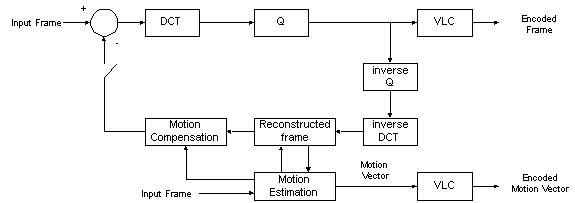
\includegraphics[width=17cm]{../images/HybridMCDCTEncoder.png}\\
 \caption{Hybrid MC DCT Encoder}
\end{figure}
\end{center}

\begin{center}
\begin{figure}[ht]  
  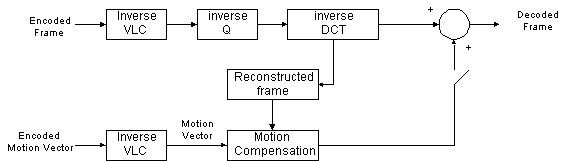
\includegraphics[width=17cm]{../images/HybridMCDCTDecoder.png}\\
 \caption{Hybrid MC DCT Decoder}
\end{figure}
 
\end{center}

\newpage

\section{Motion Estimation}

\subsection{List of Matlab cods}

\begin{itemize}
\item mefull.m - Motion Estimation using Exhaustive (Full) Block Matching algorithm
\item demo\_mefull.m - run
\end{itemize}

\subsection{Results}



 \begin{center}
  \begin{figure}[ht]
  \begin{tabular}{@{} cc @{}}

  \begin{minipage}{0.5\hsize}
   \begin{center}
   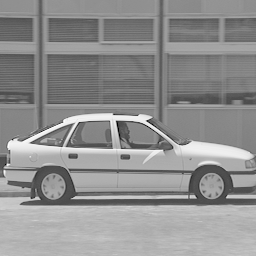
\includegraphics[width=5cm]{../images/car1.png}\\
   (a) reference frame
   \end{center}
  \end{minipage}    &
  \begin{minipage}{0.5\hsize}
   \begin{center}
   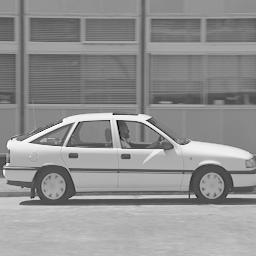
\includegraphics[width=5cm]{../images/car2.png}\\
   (b) current frame
   \end{center}
  \end{minipage}  
  \end{tabular}
 \caption{Input Images}
 \end{figure} 
\end{center}


\begin{figure}[ht]
\begin{center}
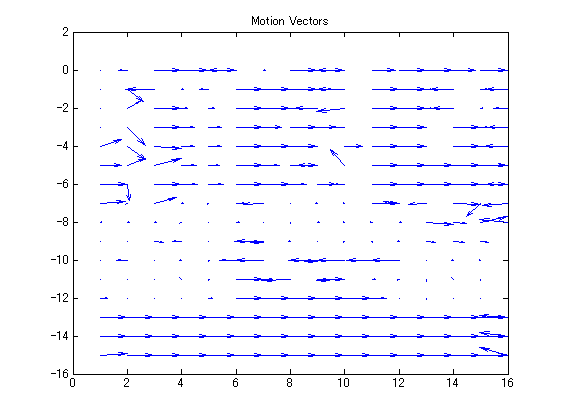
\includegraphics[width=11cm]{../images/motionfield.png}
\end{center}
\caption{Motion Vectors}
\end{figure}

\newpage

\section{Motion Compensation}

\subsection{List of Matlab codes}

\begin{itemize}
\item mc.m - Motion Compensation
\item demo\_mc.m - run
\end{itemize}
\subsection{Results}

 \begin{center}
  \begin{figure}[ht]
  \begin{tabular}{@{} cc @{}}

  \begin{minipage}{0.5\hsize}
   \begin{center}
   \includegraphics[width=10cm]{../images/estimatedCar2.png}
   \end{center}
  \end{minipage}    &
  \begin{minipage}{0.5\hsize}
   \begin{center}
   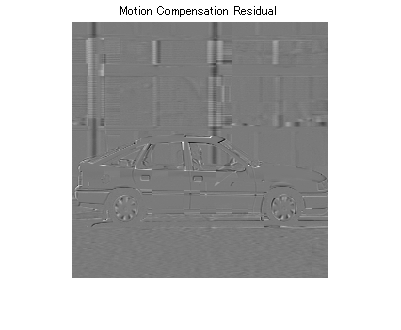
\includegraphics[width=10cm]{../images/mcresidual.png}
   \end{center}
  \end{minipage}  
  \end{tabular}
 \end{figure} 
\end{center}

 \begin{center}
  \begin{tabular}{@{} |c|c|c| @{}}
  \hline
  Time (sec) for Motion Estimation & 0.894014  \\
  \hline
  MAD & 5.260040 \\
  \hline
  \end{tabular}
\end{center}

\newpage

\section{Fast Motion Estimation via 3-step search}

\subsection{List of Matlab codes}

\begin{itemize}
\item mc3step.m - Motion Estimation using 3-step algorithm
\item demo\_mc3step.m - run
\end{itemize}

\subsection{Results}

 \begin{center}
  \begin{tabular}{@{} |c|c|c| @{}}
  \hline
  Time (sec) & 0.028770 \\
  \hline
  MAD & 5.423935 \\
  \hline
  \end{tabular}
\end{center}


\begin{figure}[ht]
\begin{center}
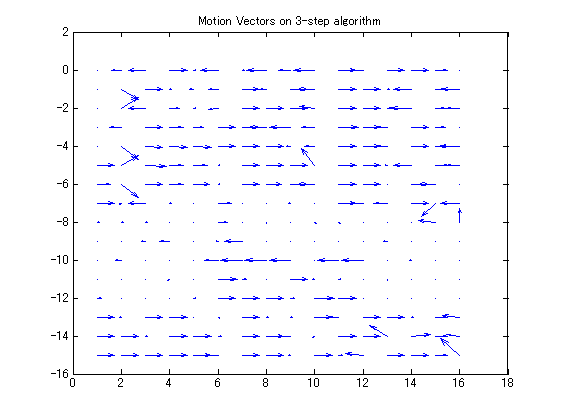
\includegraphics[width=11cm]{../images/motionfield3step.png}
\end{center}
\end{figure}

 \begin{center}
  \begin{figure}[ht]
  \begin{tabular}{@{} cc @{}}

  \begin{minipage}{0.5\hsize}
   \begin{center}
   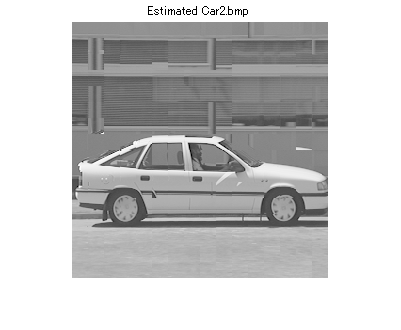
\includegraphics[width=10cm]{../images/estimatedcar23step.png}
   \end{center}
  \end{minipage}    &
  \begin{minipage}{0.5\hsize}
   \begin{center}
   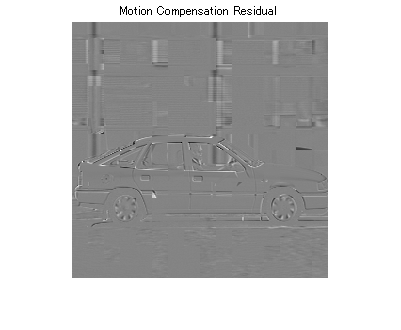
\includegraphics[width=10cm]{../images/mcresidual3step.png}
   \end{center}
  \end{minipage}  
  \end{tabular}
 \end{figure} 
\end{center}


\newpage
~
\newpage


\section{Comparative Studies}

\subsection{Results}

 \begin{center}
  \begin{figure}[ht]
  \begin{tabular}{@{} cc @{}}

  \begin{minipage}{0.5\hsize}
   \begin{center}
   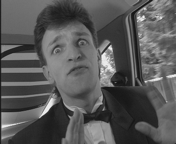
\includegraphics[width=7cm]{../images/carphone0195.png}\\
   (a) reference frame
   \end{center}
  \end{minipage}    &
  \begin{minipage}{0.5\hsize}
   \begin{center}
   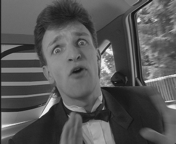
\includegraphics[width=7cm]{../images/carphone0196.png}\\
   (b) current frame
   \end{center}
  \end{minipage}  
  \end{tabular}
  \caption{Input Images}
 \end{figure} 
\end{center}

 \begin{center}
  \begin{figure}[ht]
  \begin{tabular}{@{} cc @{}}

  \begin{minipage}{0.5\hsize}
   \begin{center}
   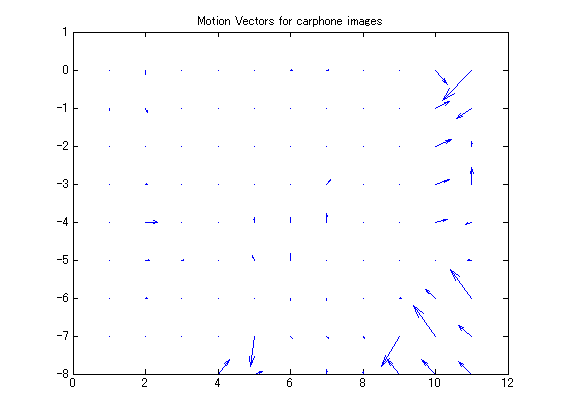
\includegraphics[width=10cm,viewport=40 20 480 320,clip]{../images/motionfieldcarphone.png}\\
      % left bottom right top
   (a) full search algorithm 
      \end{center}
  \end{minipage}    &
  \begin{minipage}{0.5\hsize}
   \begin{center}
   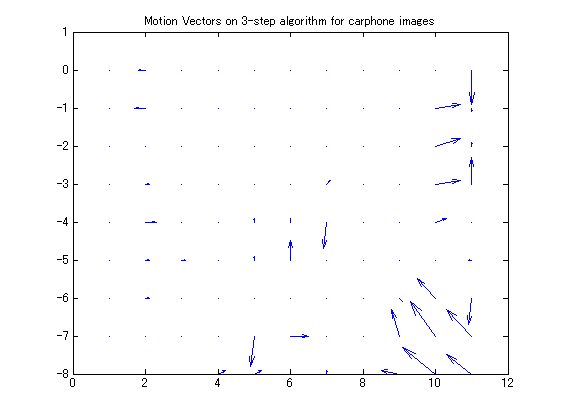
\includegraphics[width=10cm,viewport=40 20 480 320,clip]{../images/motionfield3stepcarphone.png}\\
   (b) 3-step algorithm 
      \end{center}
  \end{minipage}  
  \end{tabular}
  \caption{Motion Vectors}
 \end{figure} 
\end{center}


 \begin{center}
  \begin{figure}[ht]
  \begin{tabular}{@{} cc @{}}
  \begin{minipage}{0.5\hsize}
   \begin{center}
   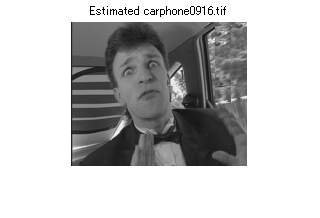
\includegraphics[width=10cm,viewport=40 40 240 160,clip]{../images/estimatedcarphone0916.png}\\
   % left bottom right top
   (a) full search algorithm
      \end{center}
  \end{minipage}    &
  \begin{minipage}{0.5\hsize}
   \begin{center}
   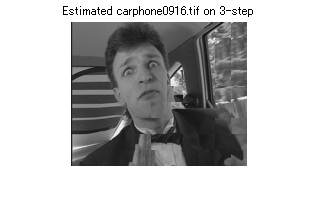
\includegraphics[width=10cm,viewport=40 40 240 160,clip]{../images/estimatedcarphone09163step.png}\\
   (b) 3-step algorithm
      \end{center}
  \end{minipage}  
  \end{tabular}
  \caption{Estimated carphone0916}
 \end{figure} 
\end{center}


\noindent
  \begin{figure}[ht]
  \begin{tabular}{cc}
  \begin{minipage}{0.5\hsize}
   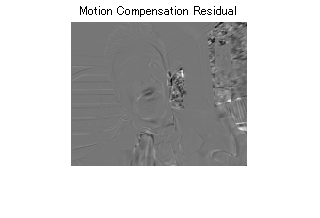
\includegraphics[width=10cm,viewport=40 40 240 160,clip]{../images/mcresidualcarphone.png}\\
      (a) full search algorithm
  \end{minipage}    &
  \begin{minipage}{0.5\hsize}
   \begin{center}
   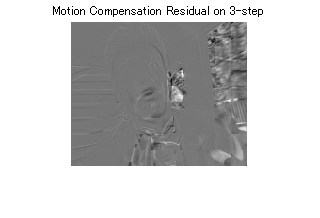
\includegraphics[width=10cm,viewport=40 40 240 160,clip]{../images/mcresidual3stepcarphone.png}\\
      (b) 3-step algorithm
      \end{center}
  \end{minipage}  
  \end{tabular}
  \caption{Motion Compensation Residual}
 \end{figure} 

\newpage

 \begin{center}
  \begin{tabular}{@{} |c|c|c| @{}}
  \hline
  & Full Search algorithm & 3-step algorithm \\
  \hline
  Time (sec) & 0.44380 & 0.03743 \\
  \hline
  MAD & 5.961293 & 7.878157 \\
  \hline
  \end{tabular}
\end{center}

\newpage

\subsubsection{Discuss the advantages and disadvantages of these two algorithms for each image sequence}

For car image sequence, there was almost no difference on MAD between full search algorithm (5.260040) and 3-step algorithm (5.423935). The computation time was 0.894014 (secs) for full search algorithm and 0.028770 (secs) for 3-step algorithm. Thus, choosing 3-step algorithm would be nice for car image sequence. 

For carphone image sequence, there was a bit big difference on MAD between full search algorithm (5.961293) and 3-step algorithm (7.878157). As the case of car image sequence, computation on 3-step algorithm was faster than computation of full search algorithm. Thus, 3-step algorithm has an advantage of computation time and a disadvantage of poor estimation compared with full search algorithm. This statement must be true for most of cases. 

\end{document}
